\begin{figure}[htp]
\centering
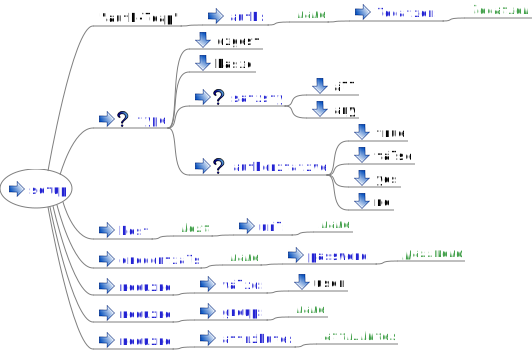
\includegraphics[width=0.8\textwidth]{httpd_setup_auth_ldap_script}
\label{fig:httpd_setup_auth_ldap_script}
\caption{Httpd LDAP Authentication Statements}
\end{figure}

%% setup auth-ldap
\TheStatement[httpd:domain:setup-auth-ldap]{setup ``auth-ldap''}
\TheStatement*[httpd!domain!setup!auth-ldap]{setup ``auth-ldap'', auth: \Arg{name}, location: \Arg{location}, \{ type host credentials require \}}

Configures authentication with a LDAP server as the storage for groups and users,
with the \Arg{name} of the authentication and the \Arg{location} that is 
restricted.

\begin{lstlisting}[style=Java]
httpd {
    domain "test1.com", address: "192.168.0.50", {
        setup "auth-ldap", auth: "Private Directory", location: "/private", {
        }
    }
}
\end{lstlisting}

%% type
\TheStatement[httpd:domain:setup-auth-ldap-type]{type}
\TheStatement*[httpd!domain!setup!auth-ldap!type]{type digest|basic [, satisfy: all|any] [, authoritative: true | false | yes | no]}

The \qcode{type} statement sets the authentication types. The 
authentication can be 
\begin{asparaitem}
\item \qcode{digest} MD5 digest authentication;
\item \qcode{basic} HTTP basic authentication;
\end{asparaitem}

The \qcode{satisfy} statement sets the criteria that must be satisfied to 
allow access to a resource.
\begin{asparaitem}
\item \qcode{all} all criteria must be met;
\item \qcode{any} only one criteria must be met;
\end{asparaitem}

The \qcode{authoritative} statement sets whether or not the authentication
is authoritative for this location.
\begin{asparaitem}
\item \qcode{true} or \qcode{yes} that it is authoritative;
\item \qcode{any} or \qcode{no} that it is not authoritative;
\end{asparaitem}

\begin{lstlisting}[style=Java]
httpd {
    domain "test1.com", address: "192.168.0.50", {
        setup "auth-ldap", auth: "Private Directory", location: "/private", {
            type AuthType.basic, satisfy: SatisfyType.any, authoritative: no
        }
    }
}
\end{lstlisting}

%% host
\TheStatement[httpd:domain:setup-auth-ldap-host]{host}
\TheStatement*[httpd!domain!setup!auth-ldap!host]{host \Arg{host}, url: \Arg{name}}

Sets the LDAP \Arg{host} and the distinguish \Arg{name} to requests the
valid groups and users.

\begin{lstlisting}[style=Java]
httpd {
    domain "test1.com", address: "192.168.0.50", {
        setup "auth-ldap", auth: "Private Directory", location: "/private", {
            host "ldap://127.0.0.1:389", url: "o=deventorg,dc=ubuntutest,dc=com?cn"
        }
    }
}
\end{lstlisting}

%% credentials
\TheStatement[httpd:domain:setup-auth-ldap-credentials]{credentials}
\TheStatement*[httpd!domain!setup!auth-ldap!credentials]{credentials \Arg{name}, password: \Arg{password}}

Sets the LDAP credentials distinguish \Arg{name} and the needed \Arg{password}.

\begin{lstlisting}[style=Java]
httpd {
    domain "test1.com", address: "192.168.0.50", {
        setup "auth-ldap", auth: "Private Directory", location: "/private", {
            credentials "cn=admin,dc=ubuntutest,dc=com", password: "adminpass"
        }
    }
}
\end{lstlisting}

%% require attribute
\TheStatement[httpd:domain:setup-auth-ldap-require attribute]{require attribute}
\TheStatement*[httpd!domain!setup!auth-ldap!require attribute]{require attribute: \Arg{attributes}}

Sets the LDAP \Arg{attributes} that are required.

\begin{lstlisting}[style=Java]
httpd {
    domain "test1.com", address: "192.168.0.50", {
        setup "auth-ldap", auth: "Private Directory", location: "/private", {
            require attribute: [group: "uniqueMember"]
            require attribute: [dn: no]
        }
    }
}
\end{lstlisting}

%% require valid
\TheStatement[httpd:domain:setup-auth-ldap-require valid]{require valid}
\TheStatement*[httpd!domain!setup!auth-ldap!require valid]{require valid: user}

See the \Statement*[httpd:domain:setup-auth-file-require-valid]{require valid}
from the \qcode{auth-file} statement.

%% require group
\TheStatement[httpd:domain:setup-auth-ldap-require group]{require group}
\TheStatement*[httpd!domain!setup!auth-ldap!require group]{require group: \Arg{name}}

Sets the required  group \Arg{name}.

\begin{lstlisting}[style=Java]
httpd {
    domain "test1.com", address: "192.168.0.50", {
        setup "auth-ldap", auth: "Private Directory", location: "/private", {
            require group: "admin1"
        }
    }
}
\end{lstlisting}
